\section{What a Simple Code Teaches Us}

\subsection{The Communication System}

The repetition code from the introduction already contains every part of a basic communication system. Alice begins with a message, changes it into a form that can resist noise (encoding), and sends it through a channel. Bob observes the channel output and tries to reconstruct the message (decoding). We can summarize this process as
\[
\mathbf{u}
\xrightarrow{\text{encoder }E}
\mathbf{x}
\xrightarrow{\text{channel}}
\mathbf{y}
\xrightarrow{\text{decoder }D}
\hat{\mathbf{u}}.
\]

Suppose the message contains $k$ bits. We write it as a vector $\mathbf{u}=(u_1,\ldots,u_k)\in\{0,1\}^k$. The encoder is a function
\[
E:\{0,1\}^k\longrightarrow\{0,1\}^n
\]
that maps $\mathbf{u}$ to an $n$-bit \emph{codeword} $\mathbf{x}=E(\mathbf{u})$. The encoder must assign different codewords to different messages; otherwise, Bob could not distinguish those messages even if the channel introduced no errors. The set of all possible codewords is the \emph{codebook}
\[
\mathcal{C}=\{E(\mathbf{u}):\mathbf{u}\in\{0,1\}^k\}.
\]
The notation $|S|$ means the number of elements in a finite set $S$. There are $2^k$ possible binary messages, so an encoder that assigns one distinct codeword to each message produces $|\mathcal{C}|=2^k$ codewords. For the redundant codes studied here, $n>k$. The full space $\{0,1\}^n$ then contains $2^n$ possible length-$n$ words, which is much larger than the codebook. Nevertheless, only $2^k$ of those words can be valid codewords because Alice has only $2^k$ possible messages to encode:
\[
\mathcal{C}\subsetneq\{0,1\}^n,
\qquad
|\mathcal{C}|=2^k<2^n.
\]
The remaining length-$n$ words are not assigned to messages. This unused space is what allows valid codewords to be separated from one another and will become essential when we discuss minimum-distance decoding.

The channel may change some components of $\mathbf{x}$ and produce a received word $\mathbf{y}\in\{0,1\}^n$. The decoder is a function $D:\{0,1\}^n\to\{0,1\}^k$ that uses $\mathbf{y}$ to form an estimate $\hat{\mathbf{u}}=D(\mathbf{y})$. In triple repetition, for example, $k=1$, $n=3$, $E(0)=000$, $E(1)=111$, and $D$ uses majority decoding.

It is useful to distinguish two kinds of error. A \emph{bit error} occurs in the channel whenever some received bit $y_i$ differs from the transmitted bit $x_i$. A \emph{block-decoding error} occurs when Bob's final estimate $\hat{\mathbf{u}}$ differs from the entire original message $\mathbf{u}$. These events are not the same: the received word $101$ contains one bit error relative to $111$, but majority decoding still recovers the correct message.

\subsection{A Precise Noise Model: The Binary Symmetric Channel}

Real channels may suffer from many different forms of interference, but a simpler model lets us isolate the main coding problem. In the \emph{binary symmetric channel} with crossover probability $p$, written $\operatorname{BSC}(p)$, both the input $X$ and the output $Y$ are bits. The channel flips the input with probability $p$ and leaves it unchanged with probability $1-p$.

An economical way to write the model is
\begin{equation}
Y=X\oplus Z,
\qquad
Z\sim\operatorname{Bern}(p),
\label{eq:bsc-model}
\end{equation}
where $\oplus$ denotes XOR, or addition modulo $2$. Thus $X\oplus0=X$ and $X\oplus1$ is the opposite bit. The notation $Z\sim\operatorname{Bern}(p)$ means
\[
\Pr(Z=1)=p,
\qquad
\Pr(Z=0)=1-p.
\]
The noise bit $Z$ therefore records whether a flip occurred.

\begin{figure}[htbp]
    \centering
    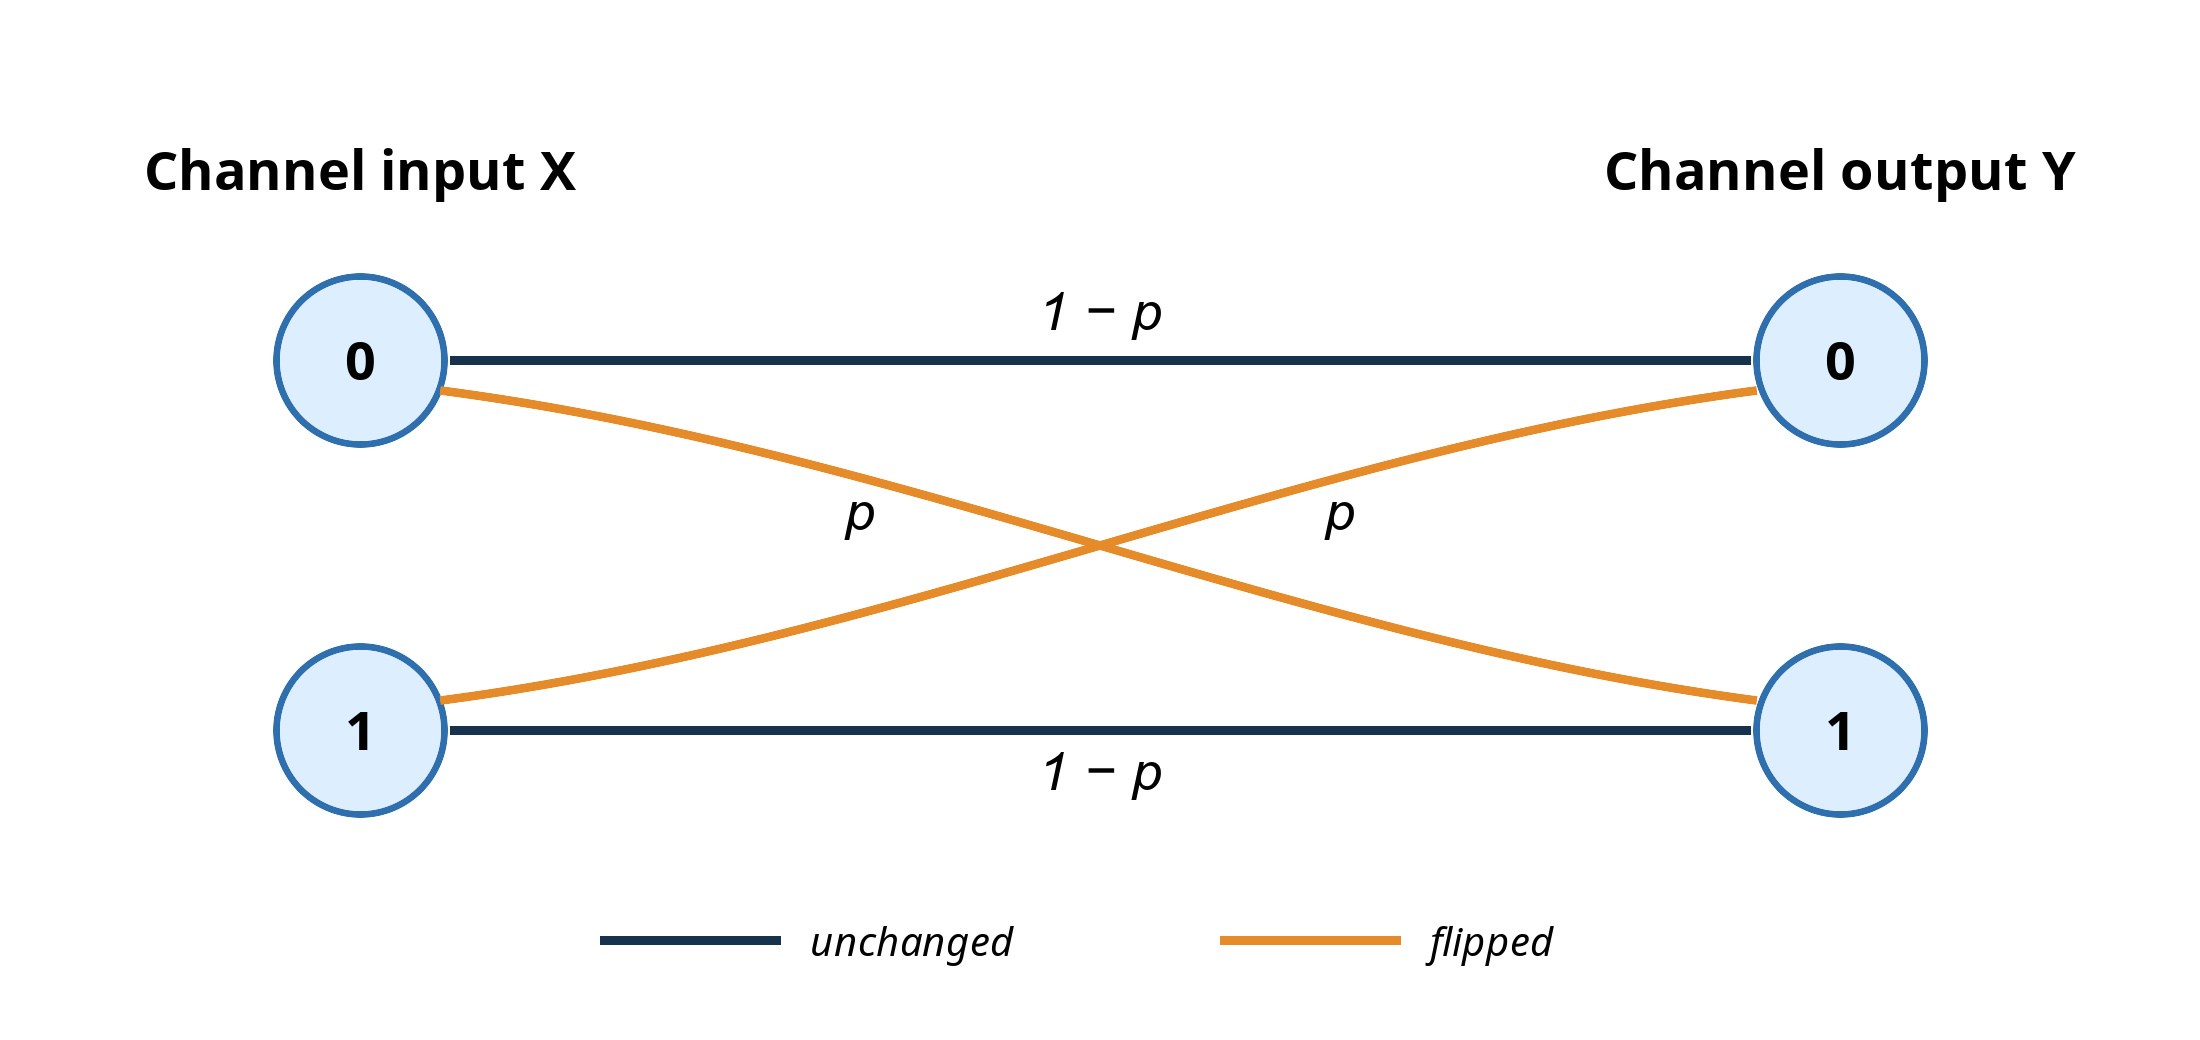
\includegraphics[width=0.78\linewidth]{assets/bsc_diagram.png}
    \caption{A $\operatorname{BSC}(p)$. Straight arrows represent an unchanged bit with probability $1-p$, while crossing arrows represent a flip with probability $p$.}
    \label{fig:bsc-model}
\end{figure}

For an $n$-bit codeword, we use the channel $n$ times and write
\[
\mathbf{y}=\mathbf{x}\oplus\mathbf{z}.
\]
Here the XOR is applied component by component. The noise bits $Z_1,\ldots,Z_n$ are assumed to be independent, each with the same probability $p$ of equaling $1$. In other words, knowing what happened to an earlier bit does not change the probabilities for the current bit. This is the \emph{memoryless} assumption. The channel is called \emph{symmetric} because a $0$ is flipped to $1$ with the same probability that a $1$ is flipped to $0$.

\newpage

Why do we normally restrict $p$ to the range $0\leq p\leq 1/2$? If $p=0$, the channel is perfect. If $p=1/2$, the two possible outputs are equally likely no matter which bit Alice sends, so Bob receives no clue about the input. Finally, if $p>1/2$, Bob can flip every received bit himself. The resulting bit is wrong with probability $1-p<1/2$, making the original channel equivalent to an easier one in our chosen range. Notice that this explanation uses only the behavior of the channel; we do not need a definition of information yet.

The BSC is one example of a \emph{discrete memoryless channel}: a channel with finite input and output alphabets whose output probabilities depend only on the current input. We will use the BSC for our discussion of Shannon's theorem. Later, the binary erasure channel will provide a more transparent worked example of polarization.

\subsection{Rate and the Redundancy Trade-Off}

The encoder begins with $k$ message bits and produces $n$ transmitted bits. The \emph{rate} of the code is
\begin{equation}
R=\frac{k}{n}.
\label{eq:code-rate}
\end{equation}
It measures the number of message bits carried per transmitted bit. Uncoded transmission has $n=k$ and rate $R=1$, but it adds no protection. Triple repetition uses three channel inputs for every message bit, so $n=3k$ and $R=1/3$.

This is the price of redundancy: when more transmitted bits are used to represent the same message, the rate decreases. However, a lower rate does not automatically produce a better code. Compare the repetition code
\[
0\longmapsto000,
\qquad
1\longmapsto111
\]
with the equally long encoding
\[
0\longmapsto000,
\qquad
1\longmapsto001.
\]
Both codes have rate $1/3$, but a single flip in the final position can change $000$ into $001$. The second code therefore cannot reliably correct even one error. What matters is not only how much redundancy is added, but also how that redundancy separates the possible codewords. Because $n>k$, the encoder has $2^n$ available locations for only $2^k$ codewords; a good encoder uses this extra room to keep the codewords apart. Hamming distance makes this idea precise.

\subsection{Hamming Distance and Minimum-Distance Decoding}

The codewords $000$ and $111$ differ in all three positions. This count is their \emph{Hamming distance}. In general, the Hamming distance between two binary words of the same length is
\[
d_H(\mathbf{x},\mathbf{x}')
=\big|\{i:x_i\neq x_i'\}\big|.
\]
The \emph{Hamming weight} $\operatorname{wt}(\mathbf{x})$ is the number of $1$s in $\mathbf{x}$. Equivalently,
\[
d_H(\mathbf{x},\mathbf{x}')
=\operatorname{wt}(\mathbf{x}\oplus\mathbf{x}').
\]
The minimum distance of a code is the smallest distance between two distinct codewords:
\begin{equation}
d_{\min}=\min_{\substack{\mathbf{x},\mathbf{x}'\in\mathcal{C}\\
\mathbf{x}\neq\mathbf{x}'}}
d_H(\mathbf{x},\mathbf{x}').
\label{eq:minimum-distance}
\end{equation}
For a linear code over a finite field $\mathbb{F}_q$, the notation $[n,k,d]_q$ records its codeword length $n$, message dimension $k$ (original message length), and minimum distance $d$ and base $q$. Such a code contains $q^k$ codewords. For a binary linear code, $q=2$ and the subscript is often omitted, giving $[n,k,d]$. The next subsection will illustrate finite-field arithmetic and linearity in the binary case. Triple repetition is therefore a $[3,1,3]_2$ code, or simply a $[3,1,3]$ binary linear code.

Distance also suggests a decoding rule. Suppose Alice transmits $111$ and Bob receives $101$. We calculate
\[
d_H(101,111)=1,
\qquad
d_H(101,000)=2.
\]
In general, a \emph{maximum-likelihood decoder} chooses the candidate codeword that makes the observed channel output most probable:
\[
\hat{\mathbf{x}}_{\mathrm{ML}}
=\underset{\mathbf{c}\in\mathcal{C}}{\operatorname{arg\,max}}
\Pr(\mathbf{Y}=\mathbf{y}\mid\mathbf{X}=\mathbf{c}).
\]
The calculation becomes especially simple on a $\operatorname{BSC}(p)$. If a candidate codeword $\mathbf{c}$ lies at Hamming distance $a$ from $\mathbf{y}$, then exactly those $a$ positions would have needed to flip, an event with probability
\[
p^a(1-p)^{n-a}.
\]
Because $p<1-p$, a candidate requiring fewer flips is more likely than one requiring more flips. Therefore, on the BSC, maximum-likelihood decoding is exactly \emph{minimum-distance decoding}:
\[
\hat{\mathbf{x}}
=\underset{\mathbf{c}\in\mathcal{C}}{\operatorname{arg\,min}}
d_H(\mathbf{y},\mathbf{c}).
\]
For the received word $101$, this rule selects $111$. The equivalence is a special property of the BSC and other symmetric error models; for a general channel, the closest word in Hamming distance need not be the most likely one.

Although Hamming space is discrete rather than Euclidean, schematic circles can help us visualize its decoding regions. The \emph{Hamming ball} of radius $t$ around a word $\mathbf{x}$ contains every binary word at distance at most $t$ from $\mathbf{x}$. For the repetition code, the two radius-one balls are
\begin{align*}
B_1(000)&=\{000,001,010,100\},\\
B_1(111)&=\{111,110,101,011\}.
\end{align*}
They do not overlap. Thus every received word containing at most one error lies in a unique ball and can be corrected to its center.

\begin{figure}[htbp]
    \centering
    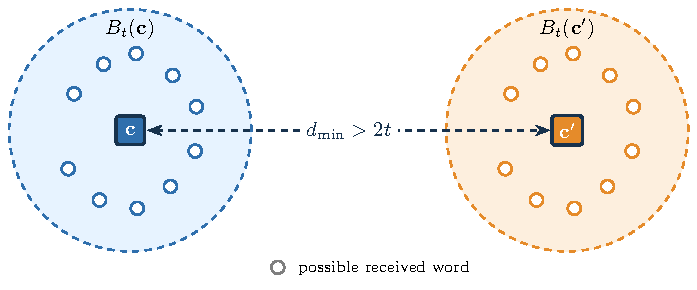
\includegraphics[width=0.9\linewidth]{assets/hamming_balls_discrete.pdf}
    \caption{Two discrete decoding regions of radius $t$ in Hamming space. The squares are codewords, and the small circles are possible received words. If the minimum distance satisfies $d_{\min}>2t$, a received word caused by at most $t$ errors belongs to at most one such region.}
    \label{fig:hamming-balls-distance}
    % \par\medskip
    % {\color{red}\small\textbf{Author revision note:} The final figure should show two schematic, nonoverlapping discrete Hamming balls $B_t(\mathbf{c})$ and $B_t(\mathbf{c}')$. Label the square centers as valid codewords and use discrete points for possible received words. Clearly show $d_{\min}>2t$ between the centers without overlapping any line or boundary. The caption should state that the circular boundaries are schematic rather than literal Euclidean geometry.\par}
\end{figure}

This picture gives two general guarantees. A code with minimum distance $d$ is guaranteed to
\[
\text{detect any pattern of up to }d-1\text{ errors},
\qquad
\text{correct any pattern of up to }
\left\lfloor\frac{d-1}{2}\right\rfloor
\text{ errors}.
\]
The floor notation $\lfloor r\rfloor$ means the greatest integer less than or equal to $r$. It appears here because the number of errors must be a whole number.
The detection statement follows because fewer than $d$ flips cannot turn one valid codeword into another. For correction, the radius-$t$ balls around distinct codewords must be disjoint, which requires $2t<d$. Triple repetition, with $d=3$, can therefore detect up to two errors or correct up to one error. By contrast, the alternative code $\{000,001\}$ has minimum distance $1$ and has no guaranteed error correction despite using the same number of transmitted bits. Redundancy provides room to separate codewords, but the encoder must use that room well.

\subsection{Why Linear Structure Is Useful}

Listing every codeword and comparing each one with the received word is one direct way to perform minimum-distance decoding. This is possible for triple repetition, but it becomes impractical when $k$ is large because the codebook contains $2^k$ words. A useful code therefore needs a concise structure. Polar codes belong to the important family of \emph{linear codes}, whose encoding can be described by matrix multiplication.

The entries of these matrices belong to the binary field $\mathbb{F}_2=\{0,1\}$. Addition in $\mathbb{F}_2$ is XOR, so $1+1=0$, while multiplication follows the usual binary rules. A binary code $\mathcal{C}\subseteq\mathbb{F}_2^n$ is linear if it is a vector subspace. Concretely, the all-zero word belongs to $\mathcal{C}$, and the XOR of any two codewords is another codeword.

\begin{figure}[htbp]
    \centering
    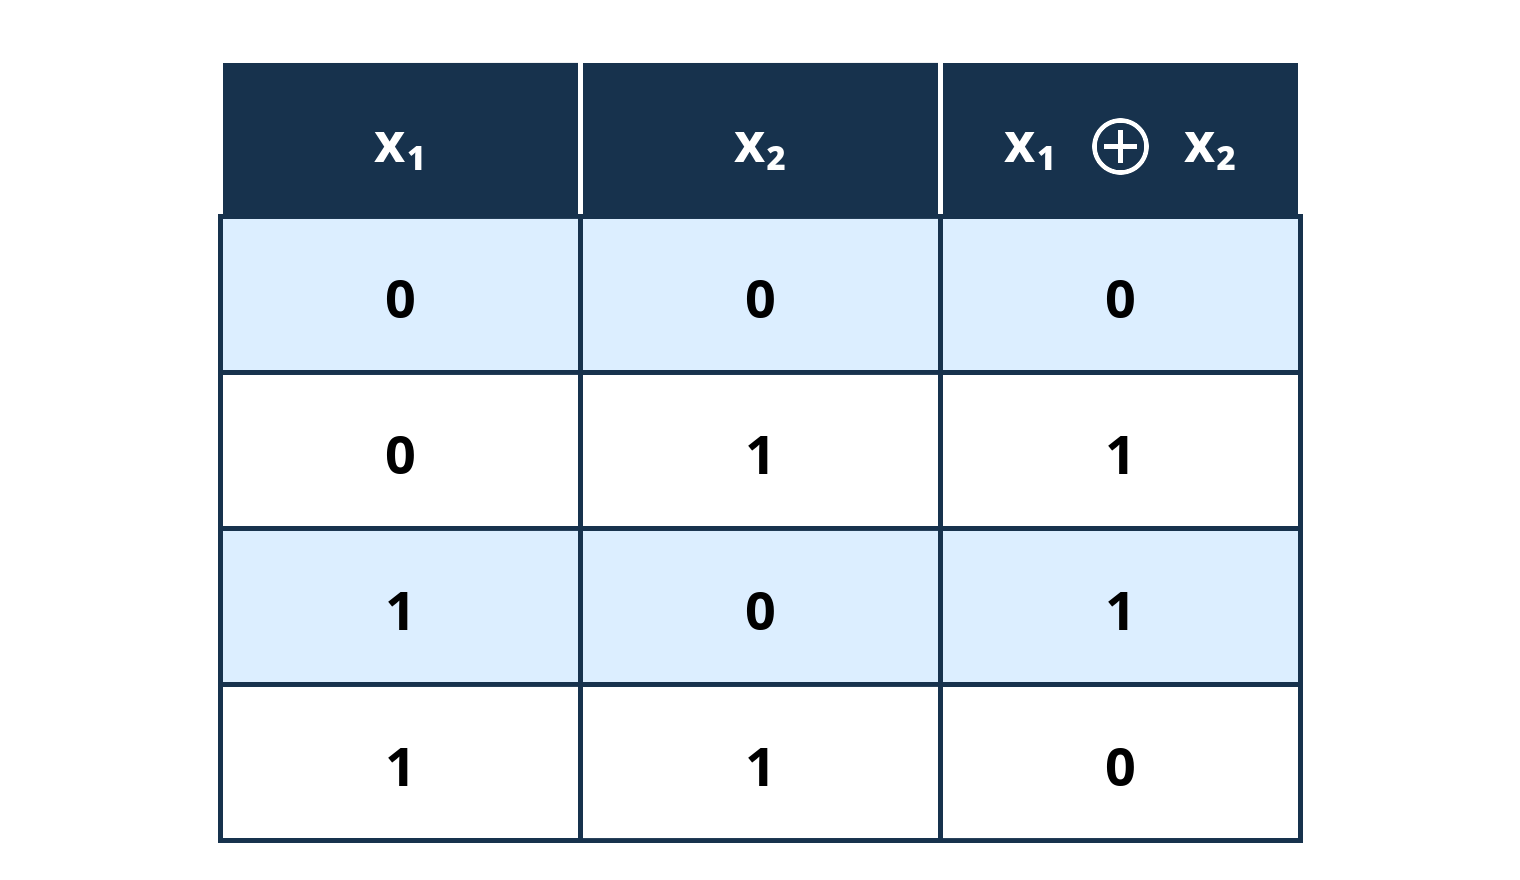
\includegraphics[width=0.52\linewidth]{assets/xor_truth_table.png}
    \caption{Truth table for XOR, the addition operation in $\mathbb{F}_2$. Its output is $1$ exactly when the two input bits differ.}
    \label{fig:xor-table}
\end{figure}

A linear encoder can be specified by a full-row-rank $k\times n$ \emph{generator matrix} $G$. Treating the message as a row vector, encoding becomes
\begin{equation}
\mathbf{x}=\mathbf{u}G,
\label{eq:generator-encoding}
\end{equation}
where every operation is performed in $\mathbb{F}_2$. For triple repetition,
\[
G=\begin{bmatrix}1&1&1\end{bmatrix}.
\]
The message $u=0$ produces $0G=000$, while $u=1$ produces $1G=111$. The same description that previously required two separate encoding rules has become one matrix operation.

Linear codes can also be described by a \emph{parity-check matrix} $H$. A word $\mathbf{x}$ is a valid codeword exactly when $H\mathbf{x}^{T}=\mathbf{0}$. If $G$ and $H$ describe the same code, then $HG^{T}=0$. Parity-check matrices are valuable in many coding methods, but the polar-code construction later in this paper will be easier to follow through its generator matrix.

The first step of that construction will combine two bits according to
\[
(u_1,u_2)\longmapsto(u_1\oplus u_2,u_2).
\]
This operation is itself linear, since
\[
\begin{bmatrix}u_1&u_2\end{bmatrix}
\begin{bmatrix}
1&0\\
1&1
\end{bmatrix}
=
\begin{bmatrix}u_1\oplus u_2&u_2\end{bmatrix}.
\]
We have therefore developed the language needed to describe codes and their reliability. What remains is the larger question posed in the introduction: for a channel such as the BSC, how high can the rate be while the decoding error still becomes increasingly unlikely?
